\documentclass[10pt]{beamer}
\usepackage{listings}

\usepackage{amsmath}
\usetheme[progressbar=frametitle]{metropolis}
\usepackage{appendixnumberbeamer}

\usepackage{booktabs}
\usepackage[scale=2]{ccicons}

\usepackage{pgfplots}
\usepgfplotslibrary{dateplot}

\usepackage{xspace}
\newcommand{\themename}{\textbf{\textsc{metropolis}}\xspace}

\title{Algorithmic Journeys}
\subtitle{Generic algorithms and performance}
% \date{\today}
\date{}
\author{Taras Shevhcnkeo}
\institute{Rails Reactor}
% \titlegraphic{\hfill\includegraphics[height=1.5cm]{logo.pdf}}

\begin{document}

\maketitle

\begin{frame}{Table of contents}
  \setbeamertemplate{section in toc}[sections numbered]
  \tableofcontents[hideallsubsections]
\end{frame}

\section{Terminology}

\begin{frame}[fragile]{Terminology}
  \begin{enumerate}
    \item Datum
    \item Value
    \item Value type
    \item Object
    \item Object type
  \end{enumerate}
\end{frame}



\begin{frame}[fragile]{Datum}
\begin{block}{Definition}
A \textbf{datum} is a sequence of bits.
\end{block}

\begin{block}{Example}
01000001 is an example of a datum.
\end{block}

\end{frame}

\begin{frame}[fragile]{Value}
\begin{block}{Definition}
A \textbf{value is} a \textbf{datum} together with its interpretation.
\end{block}
\begin{block}{Example}
The \textbf{datum} 01000001 might have the interpretation of the integer 65, or the character “A".
\end{block}
\begin{block}{Explanation}
Every \textbf{value} must be associated with a \textbf{datum} in memory; there is no way to refer to disembodied \textbf{values} in modern programming languages.
\end{block}
\end{frame}

\begin{frame}[fragile]{Value type}
\begin{block}{Definition}
A \textbf{value type} is a set of values sharing a common interpretation.
\end{block}
\end{frame}

\begin{frame}[fragile]{Object}
\begin{block}{Definition}
An \textbf{object} is a collection of bits in memory that contain a \textbf{value} of a given \textbf{value type}.
\end{block}
\begin{block}{Explanation}
An \textbf{object} is immutable if the value never changes, and mutable otherwise. An object is unrestricted if it can contain any \textbf{value} of its \textbf{value type}.
\end{block}
\end{frame}


\begin{frame}[fragile]{Object type}
\begin{block}{Definition}
An \textbf{object type} is a uniform method of storing and retrieving \textbf{values} of a given \textbf{value type} from a particular \textbf{object} when given its address.
\end{block}
\end{frame}


\section{Programming with concepts}

\begin{frame}{Basic idea}
\begin{block}{}
The essence of generic programming lies in the idea of concepts. A concept is a way of describing a family of related object types.
\end{block}
\begin{center}
    \begin{tabular}{ | p{1.5cm} | l | l | p{3cm} |}
    \hline
    \textbf{Natural Science} & \textbf{Mathematics} & \textbf{Programming} & \textbf{Programming Examples} \\ \hline
      genus & theory & concept & Integral, Character \\
      species & model & type or class & uint8\_t, char \\
      invidiual & element & instance  & 01000001(65, 'A') \\
    \hline
    \end{tabular}
\end{center}
\end{frame}

\begin{frame}{Notion of Regularity}
\begin{block}{Operation}
  \begin{enumerate}
    \item Copy construction
    \item Assignment
    \item Equality
    \item Destruction
  \end{enumerate}
\end{block}
\begin{block}{Semantic}
    $$\forall a ~ \forall b ~ \forall c : T~a(b)  \implies(b = c \implies a = c)$$
    $$\forall a ~ \forall b ~ \forall c : a \leftarrow b  \implies(b = c \implies a = c)$$
    $$\forall f \in RegularFunction: a = b \implies f(a) = f(b)$$
\end{block}
\end{frame}

\begin{frame}{More examples of concepts}
\begin{enumerate}
  \item Regular Type
  \item Semiegular Type
  \item Functional Procedure
  \item Homogeneous Function
  \item Homogeneous Predicate
  \item Semiring
  \item Sequence
  \item Totally Ordered
  \item Input Iterator
  \item Forfward Iterator
  \item Bidirectional Iterator
\end{enumerate}
\end{frame}

\begin{frame}{Properties}
\begin{enumerate}
  \item Associative
  \item Distributive
  \item Transitive
  \item Semiegular Type
  \item Functional Procedure
\end{enumerate}
\end{frame}

\begin{frame}{Techniques}
\begin{enumerate}
  \item Transformation-action duality
  \item Operation-accumulation procedure duality
  \item Memory adaptivity
  \item Reduction to constrained subproblem 
\end{enumerate}
\end{frame}

\section{Egyptian multiplication}

\begin{frame}{Simple algorithm}
  \begin{columns}
    \column{0.5\textwidth}
      \centering{3 * 8}
      \begin{table}
        \begin{tabular}{l|r}
          \toprule
          x & y\\
          \midrule
          3 & 8\\ \hline
          6 & 7\\ \hline
          9 & 6\\ \hline
          12 & 5\\ \hline
          15 & 4\\ \hline
          18 & 3\\ \hline
          21 & 2\\ \hline
          24 & 1\\ \hline
          \bottomrule
        \end{tabular}
      \end{table}

    \column{0.5\textwidth}
      \centering{8 * 3}
      \begin{table}
        \begin{tabular}{l|r}
          \toprule
          x & y\\
          \midrule
          8 & 3\\ \hline
          16  & 2\\ \hline
          24 & 1\\ \hline
          \bottomrule
        \end{tabular}
      \end{table}
  \end{columns}
\end{frame}


\begin{frame}[fragile]{Far away from egyptian multiplication}
\begin{block}{Code}
  \lstinputlisting[language=Python]{code/intersect.py}
\end{block}
\begin{block}{Output}
\begin{lstlisting}
0
1
{1, 2}
\end{lstlisting}
\end{block}
\end{frame}

\begin{frame}[fragile]{The first implementation}
\begin{block}{Code}\lstinputlisting[language=c++]{code/0.h}\end{block}
\end{frame}

\begin{frame}[fragile]{Egyptian multiplication - 1}
\begin{block}{Code}\lstinputlisting[language=c++]{code/1.h}\end{block}
\end{frame}

\begin{frame}[fragile]{Egyptian multiplication - 2}
\begin{block}{Code}\lstinputlisting[language=c++]{code/2.h}\end{block}
\end{frame}

\begin{frame}[fragile]{Egyptian multiplication - 3}
\begin{block}{Code}\lstinputlisting[language=c++]{code/3.h}\end{block}
\end{frame}

\begin{frame}[fragile]{Egyptian multiplication - 4}
\begin{block}{Code}\lstinputlisting[language=c++]{code/4.h}\end{block}
\end{frame}

\begin{frame}[fragile]{Egyptian multiplication - 5}
\begin{block}{Code}\lstinputlisting[language=c++]{code/5.h}\end{block}
\end{frame}

\begin{frame}[fragile]{Egyptian multiplication - 6}
\begin{block}{Code}\lstinputlisting[language=c++]{code/6.h}\end{block}
\end{frame}

\begin{frame}[fragile]{Egyptian multiplication - 7}
\begin{block}{Code}\lstinputlisting[language=c++]{code/7.h}\end{block}
\end{frame}

\begin{frame}[fragile]{Egyptian multiplication - 8}
\begin{block}{Code}\lstinputlisting[language=c++]{code/8.h}\end{block}
\end{frame}

\begin{frame}[fragile]{Egyptian multiplication - 9}
\begin{block}{Code}\lstinputlisting[language=c++]{code/9.h}\end{block}
\end{frame}

\begin{frame}[fragile]{Egyptian multiplication - 10}
\begin{block}{Code}\lstinputlisting[language=c++]{code/10.h}\end{block}
\end{frame}

\begin{frame}[fragile]{Egyptian multiplication - Generic version}
\begin{block}{Code}\lstinputlisting[language=c++]{code/11.h}\end{block}
\end{frame}

\begin{frame}[fragile]{Egyptian multiplication - Generic version}
\begin{block}{Code}\lstinputlisting[language=c++]{code/12.h}\end{block}
\end{frame}

\begin{frame}[fragile]{Applications of Egyptian Multiplication}
  \begin{enumerate}
    \item Multiplication
    \item Pow
    \item Transitive closure
    \item Shortest path
  \end{enumerate}
\end{frame}

\begin{frame}[fragile]{Multiplication}
  \begin{enumerate}
    \item Multiplication
    \item Pow
    \item Transitive closure
    \item Shortest path
  \end{enumerate}
\end{frame}

\begin{frame}[fragile]{Egyptian Multiplication for Multiplication}
\begin{block}{Code}\lstinputlisting[language=c++]{code/13.h}\end{block}
\end{frame}

\begin{frame}[fragile]{Egyptian Multiplication for Pow}
\begin{block}{Code}\lstinputlisting[language=c++]{code/14.h}\end{block}
\end{frame}

\begin{frame}[fragile]{Egyptian Multiplication for Transitive Closure}
\begin{block}{Code}\lstinputlisting[language=c++]{code/14.h}\end{block}
\end{frame}

\begin{frame}[fragile]{Egyptian Multiplication for Transitive Closure}
\begin{block}{Code}\lstinputlisting[language=c++]{code/15.h}\end{block}
\end{frame}

\begin{frame}[fragile]{Egyptian Multiplication for Shortest path}
\begin{block}{Code}\lstinputlisting[language=c++]{code/16.h}\end{block}
\end{frame}

\begin{frame}[fragile]{Graph}
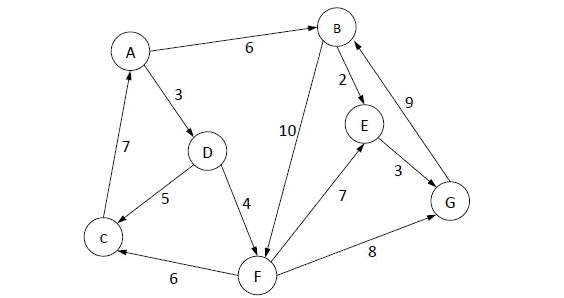
\includegraphics[height=5cm]{images/graph.png}
\end{frame}

\begin{frame}[fragile]{Graph}
\[
\begin{bmatrix}
0 &		6	&	inf	&	3	&	inf	&	inf	&	inf	\\
inf	&	0	&	inf	&	inf	&	2	&	10	&	inf	\\
7	&	inf	&	0 &		inf	&	inf	&	inf	&	inf	\\	
inf	&	inf	&	5	&	0	&	inf	&	4	&	inf		\\
inf	&	inf	&	inf	&	inf	&	0	&	inf	&	3		\\
inf	&	inf	&	6	&	inf	&	7	&	0	&	8		\\
inf &	9	 &	inf	&	inf	&	inf	&	inf	&	0 \\
\end{bmatrix}
\]
\end{frame}

\begin{frame}[fragile]{Shortest distance}
\[
\begin{bmatrix}
0	&	6	&	8	&	3	&	8	&	7	&	11		\\
23 &	0	&	16 & 26	&	2	&	10	&	5	 \\
7	&	13 &	0	&	10 & 15	&	14	&	18 \\
12 & 18	&	5	&	0	&	11	&	4	&	12 \\
inf	&	12 & 28	&	inf	&	0	&	22 &	3	\\
13 &	17 &	6	&	16 &	7	&	0	&	8	\\
32 &	9	&	25	&	inf	&	11 &	19 &	0	\\
\end{bmatrix}
\]
\end{frame}

\begin{frame}{Homework}
  \begin{enumerate}
    \item Rewrite functors as algorithms 
    \item Play around linear recurrences
  \end{enumerate}
\end{frame}


\section{Conclusion}

\begin{frame}{Conclusion}
  \begin{enumerate}
    \item Concreteness costs
    \item Abstracting algorithms to their most general setting without losing efficiency
    \item Know your algorithms
  \end{enumerate}
\end{frame}


\end{document}
